\begin{wrapfigure}[10]{r}[0pt]{100mm}
	\centering
    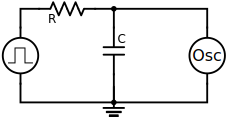
\includegraphics[width=80mm]{schema.pdf}
    \caption{Schema del circuito utilizzato.}
    \label{fig:circuito}
\end{wrapfigure}

%\begin{multicols}{2}
\section{Strumenti}

$\bullet \quad$Oscilloscopio \\
$\bullet \quad$Cablaggio\\
$\bullet \quad$Decadi di resistenze e capacità\\
$\bullet \quad$Generatore di forme d'onda\\
$\bullet \quad$Multimetro digitale\\
$\bullet \quad$Breadboard (basetta sperimentale)\\
%\columnbreak
%\begin{figure}[h!]
%	\centering
%	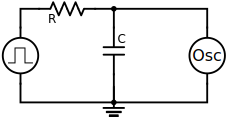
\includegraphics[width=\textwidth]{schema.pdf}
%    \caption{Schema del circuito utilizzato.}
%    \label{fig:circuito}
%\end{figure}

%\end{multicols}
\hspace{2pt}\\